\scanpage{166}

\[
\left\{\begin{aligned}
&\sigma_1^2=\sigma_2^2=(\sigma_1\sigma_2)^2=1\\
&\rho_1,\rho_{\unsure{2|\infty}}
\end{aligned}\right.
\]
\[
\sigma_i\rho_j=\rho_{\unsure{j|2}}^{-1}
\]
\[
\begin{aligned}
\widetilde\tau\widetilde\rho&=\widetilde\rho^{-1}\\
\widetilde\tau\widetilde\sigma&=\widetilde\sigma^{-1}
\end{aligned}
\qquad\widetilde\rho^3\,-
\]

\figure{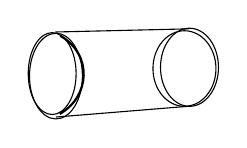
\begin{tikzpicture}[x=.8cm,y=.8cm]
\draw (0,0) ellipse (.38 and .65);
\draw (.06,-.04) ellipse (.42 and .68);
\draw (2.1,.08) ellipse (.5 and .6);
\draw (2.18,.1) ellipse (.46 and .62);
\draw (.05,.66)--(2.17,.71);\draw (.06,-.69)--(2.15,-.52);
\draw[thick] (.13,.6) .. controls (.65,.3) and (.6,-.37) .. (.12,-.64);
\end{tikzpicture}}

\figure{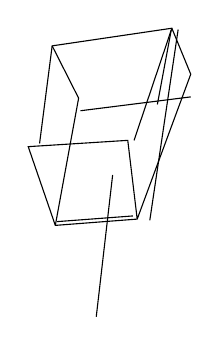
\begin{tikzpicture}[x=.8cm,y=.8cm]
\draw (-.1,.1)--(.1,1.65)--(2,1.93)--(2.3,1.2)--(1.45,-1.1)--(.15,-1.2)--(-.28,.05)--(1.3,.15)--(1.45,-1.1);
\draw (.1,1.65)--(.52,.82)--(.15,-1.2);
\draw (.55,.62)--(2.3,.84);\draw (2,1.93)--(1.4,.15);
\draw (2.1,1.91)--(1.65,-1.12);\draw (1.99,1.9)--(1.77,.72);
\draw (.18,-1.14)--(1.38,-1.05);\draw (1.06,-.4)--(.8,-2.65);
\end{tikzpicture}}

\figure{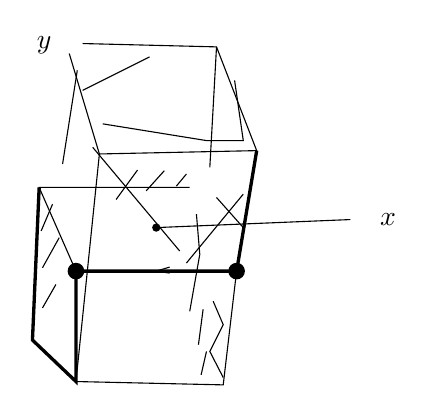
\begin{tikzpicture}[x=.85cm,y=.85cm]
\draw (0,2.9)--(.45,1.4)--(2.8,1.45)--(2.2,3)--(.2,3.05);
\draw (.12,2.65)--(-.1,1.25);
\draw (.45,1.4)--(.1,-2)--(-.55,-1.38)--(-.45,.9)--(1.8,.9);
\draw[very thick] (-.45,.9)--(-.55,-1.38)--(.1,-2)--(.1,-.35)--(2.5,-.35)--(2.8,1.45);
\draw (.1,-2)--(2.3,-2.05)--(2.5,-.35);
\draw (-.45,.9)--(.1,-.35);\draw (2.2,3)--(2.1,1.2);
\draw (.5,1.85)--(2.05,1.6)--(2.6,1.6)--(2.47,2.5);
\draw (.2,2.35)--(1.2,2.85);\draw (.35,1.5)--(1.65,-.05);
\draw (1.3,.3)--(4.2,.42);\fill (1.3,.3) circle (1.5pt);
\fill (.1,-.35) circle (3pt);\fill (2.5,-.35) circle (3pt);
\draw (1.5,-.38)--(1.3,-.35)--(1.5,-.29);
\draw (1.95,-.1)--(1.9,.5);\draw (1.95,-.1)--(1.8,-.95);
\draw (2.6,.8)--(1.75,-.23);\draw (2.2,.75)--(2.6,.3);
\draw (2.15,-.8)--(2.3,-1.15)--(2.1,-1.55)--(2.3,-1.94);
\draw (2,-.92)--(1.93,-1.45);\draw (2.05,-1.55)--(1.97,-1.9);
\draw (-.42,.25)--(-.25,.65);\draw (-.4,-.3)--(-.15,.15);\draw (-.4,-.9)--(-.2,-.55);
\draw (.7,.72)--(1.02,1.16);\draw (1.15,.85)--(1.42,1.15);\draw (1.6,.92)--(1.75,1.1);
\node[left] at (-.12,3.02) {$y$};\node[right] at (4.5,.42) {$x$};
\end{tikzpicture}}

\figure{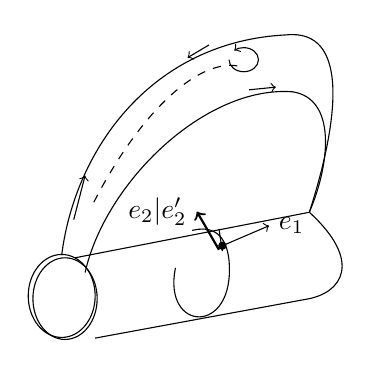
\begin{tikzpicture}[x=.85cm,y=.85cm]
\draw (0,0) ellipse (.5 and .62);
\draw (.05,-.04) ellipse (.48 and .61);
\draw (.2,.57)--(3.7,1.25) .. controls (4.5,.52) and (4.2,.04) .. (3.65,-.05)--(.5,-.63);
\draw (0,.61) .. controls (.2,2.2) and (1.35,3.8) .. (3.35,3.9)
 .. controls (4.3,4) and (4.15,2.65) .. (3.7,1.25);
\draw (.35,.35) .. controls (.65,1.7) and (2.15,3.15) .. (3.45,3.05)
 .. controls (4.1,2.95) and (4.02,2) .. (3.7,1.25);
\draw[dashed] (.48,1.4) .. controls (1.2,2.8) and (2.1,3.6) .. (2.7,3.42);
\draw[->] (.18,1.14)--(.35,1.8);\draw[->] (2.2,3.75)--(1.88,3.56);
\draw[->] (2.8,3.08)--(3.2,3.12);
\draw[->] (2.5,3.53) arc[start angle=180,end angle=490,x radius=.22,y radius=.18];
\draw (1.7,.42) .. controls (1.5,-.55) and (2.6,-.6) .. (2.5,.53)
 .. controls (2.45,1.02) and (2.15,1.03) .. (1.95,.98);
\draw[->] (2.4,.75)--(3.1,1.05) node[right] {$e_1$};
\draw[->,thick] (2.35,.69)--(2.02,1.26) node[left] {$\unsure{e_2|e'_2}$};
\draw (2.4,.67)--(2.35,1);\fill (2.4,.75) circle (1.5pt);
\end{tikzpicture}}

\[
x\mathrel{\mapstochar\! -\! -}-x\qquad
 y\longmapsto y
\]
\[
(x,y,z)\longmapsto\unsure{ix|iX},
\]
\[
(z,t)\longrightarrow(iz,-t)
\]

\figure{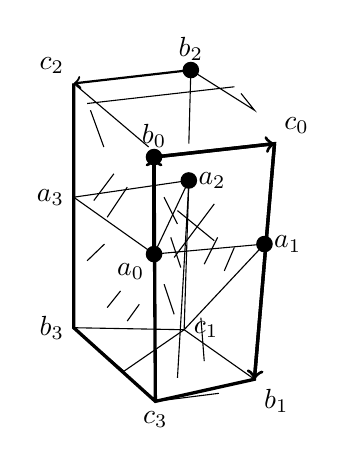
\begin{tikzpicture}[x=.85cm,y=.85cm]
\coordinate (c2) at (0,3.8);\coordinate (b2) at (1.75,4);
\coordinate (a3) at (0,2.1);\coordinate (b3) at (0,.15);
\coordinate (b0) at (1.2,2.7);\coordinate (c0) at (3,2.9);
\coordinate (a0) at (1.2,1.25);\coordinate (a1) at (2.85,1.4);
\coordinate (a2) at (1.72,2.35);\coordinate (c1) at (1.65,.12);
\coordinate (b1) at (2.7,-.62);\coordinate (c3) at (1.22,-.95);
\draw[very thick] (c2)--(b3)--(c3)--(b1)--(c0)--(b0)--(c3);
\draw[very thick,->] (b0)--(c0);\draw[very thick,->] (c0)--(b1);
\draw[very thick,->] (a0)--(b0);\draw[thick,->] (b2)--(c2);
\draw (b2)--(1.72,2.9);\draw (c2)--(1.12,2.85);\draw (b2)--(2.7,3.4)--(2.5,3.65);
\draw (a3)--(a2)--(a0)--(a1)--(c1)--(b3);\draw (a2)--(c1);
\draw (c1)--(b1);\draw (c3)--(2.17,-.83);\draw (a3)--(a0);
\draw (b3)--(.75,-.5)--(c1);\draw (.2,3.5)--(2.4,3.75);
\draw (.25,3.4)--(.45,2.85);\draw (.3,2.05)--(.6,2.45);\draw (.5,1.8)--(.8,2.25);
\draw (.2,1.15)--(.46,1.4);\draw (.5,.45)--(.7,.7);\draw (.8,.25)--(.98,.5);
\draw (1.35,2.1)--(1.55,1.7);\draw (1.45,1.5)--(1.6,1.05);
\draw (1.35,.8)--(1.5,.35);\draw (1.95,1.1)--(2.15,1.5);\draw (2.25,1)--(2.4,1.35);
\draw (1.9,.3)--(1.95,-.35);\draw (1.72,2.3)--(1.55,-.6);
\draw (1.55,1.9)--(2.1,1.45);\draw (1.5,1.2)--(2.1,2);
\foreach \p in {a0,a1,a2,b0,b2} {\fill (\p) circle (3pt);}
\node[above left] at (c2) {$c_2$};\node[above] at (b2) {$b_2$};
\node[left] at (a3) {$a_3$};\node[left] at (b3) {$b_3$};
\node[above] at (b0) {$b_0$};\node[above right] at (c0) {$c_0$};
\node[below left] at (a0) {$a_0$};\node[right] at (a1) {$a_1$};
\node[right] at (a2) {$a_2$};\node[right] at (c1) {$c_1$};
\node[below right] at (b1) {$b_1$};\node[below] at (c3) {$c_3$};
\end{tikzpicture}}

\[
\sigma\varphi
\qquad \deleted{\unsure{\mathbb Z_2|\mathbb Z/2}}\unsure{D_\sigma|D\sigma}
\]
\[
\boxed{\sigma^2=\sigma_1\sigma_2=\boxed{\sigma_2\sigma_1}}
\]
\[
\sigma_1^2=\sigma_2^2\quad(=\sigma^4)=1
\]
\[
\begin{aligned}
\sigma_1(\sigma)&=\sigma^{-1}\\
\sigma_2(\sigma)&=\sigma^{-1}
\end{aligned}\qquad ?
\]
\[
\deleted{(\sigma_1,\sigma_2)}\qquad\deleted{(\sigma_1\sigma_2)^2}
\]
\[
\begin{aligned}
\sigma(z,t)&=\unsure{(iz|(z},-t)\\
\sigma_1(z,t)&=(\overline z,t)\\
\sigma_2(z,\unsure{t|h})&=(-\overline z,t)
\end{aligned}
\]
\[
\sigma_2=\sigma_1\sigma^2=\sigma^2\sigma_1
\]
\[
\begin{pmatrix}1&1\\0&1\end{pmatrix}\qquad
\begin{pmatrix}1&-1\\0&1\end{pmatrix}
\]
\[
(z,t)\mathrel{\mapstochar\! -\! -}(\overline z,t)
 \mathrel{\mapstochar\! -\! -}(i\overline z,-t)
 \longmapsto(-iz,-t)
\]
\margin{166}
